\documentclass{article}
\usepackage{tikz}
\usetikzlibrary{shapes,arrows,positioning,fit,calc}
\usepackage{listings}
\usepackage{graphicx}
\usepackage{booktabs}

\title{Self-Hosting C Compiler: Methods, Implementation, and Bootstrap Convergence Analysis}
\author{Compiler Construction Project}
\date{\today}

\begin{document}

\maketitle

\begin{abstract}
This paper documents the implementation of a self-hosting C compiler capable of compiling itself. We present the architecture, key implementation challenges, and a detailed analysis of the bootstrap convergence process. The compiler uses a three-stage bootstrap: Stage0 (compiled by GCC), Stage1 (compiled by Stage0), and Stage2 (compiled by Stage1). We identify and fix critical bugs preventing self-compilation and measure convergence through functional testing.
\end{abstract}

\section{Introduction}

A self-hosting compiler is one that can compile its own source code. This capability demonstrates correctness and is a key milestone in compiler development. Our compiler, written in C, targets ARM64 architecture.

\subsection{Goals}
\begin{itemize}
    \item Implement a C compiler that can compile itself
    \item Achieve bootstrap convergence where Stage0 and Stage1 produce identical output
    \item Document the bug-fixing process for educational purposes
\end{itemize}

\section{Methods}

\subsection{Architecture Overview}

\begin{figure}[h]
\centering
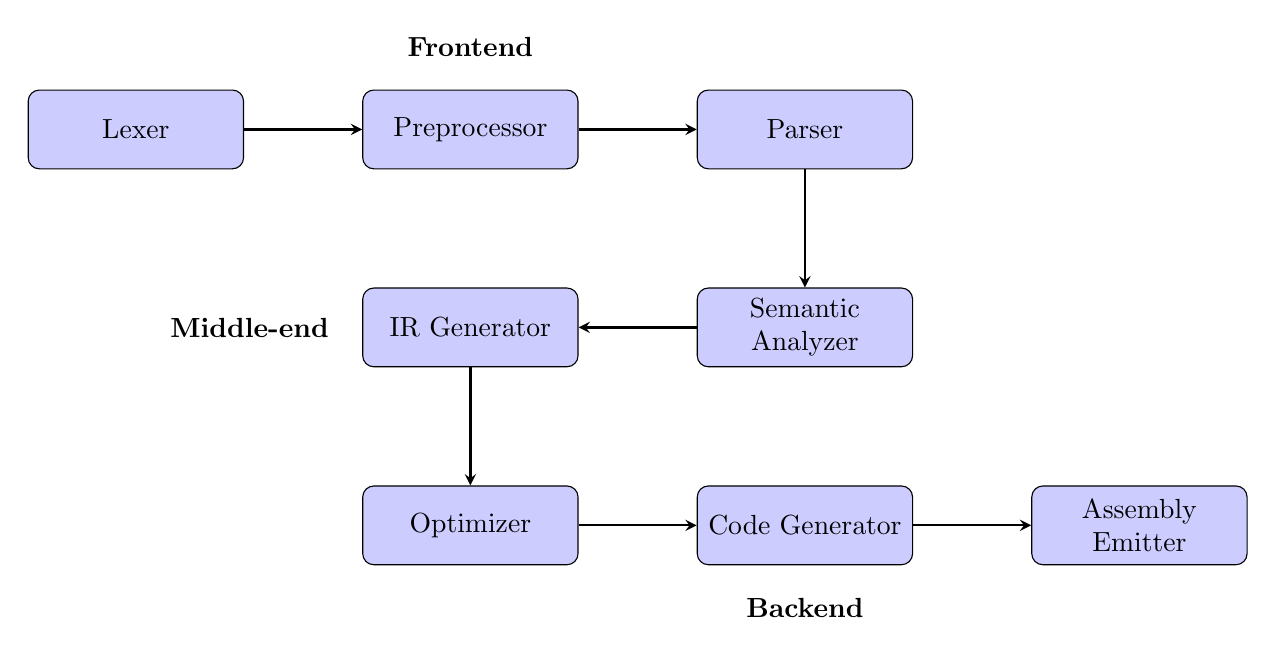
\begin{tikzpicture}[node distance=1.5cm, auto,
    block/.style={rectangle, draw, fill=blue!20, text width=2.5cm, text centered, rounded corners, minimum height=1cm},
    arrow/.style={->, >=stealth, thick}
]

% Frontend
\node[block] (lexer) {Lexer};
\node[block, right=of lexer] (preproc) {Preprocessor};
\node[block, right=of preproc] (parser) {Parser};

% Middle-end
\node[block, below=of parser] (analyzer) {Semantic Analyzer};
\node[block, left=of analyzer] (ir) {IR Generator};

% Backend
\node[block, below=of ir] (optimize) {Optimizer};
\node[block, right=of optimize] (codegen) {Code Generator};
\node[block, right=of codegen] (emit) {Assembly Emitter};

% Arrows
\draw[arrow] (lexer) -- (preproc);
\draw[arrow] (preproc) -- (parser);
\draw[arrow] (parser) -- (analyzer);
\draw[arrow] (analyzer) -- (ir);
\draw[arrow] (ir) -- (optimize);
\draw[arrow] (optimize) -- (codegen);
\draw[arrow] (codegen) -- (emit);

% Labels
\node[above=0.3cm of preproc, font=\bfseries] {Frontend};
\node[left=0.3cm of ir, font=\bfseries] {Middle-end};
\node[below=0.3cm of codegen, font=\bfseries] {Backend};

\end{tikzpicture}
\caption{Compiler Pipeline Architecture}
\end{figure}

\subsection{Bootstrap Process}

\begin{figure}[h]
\centering
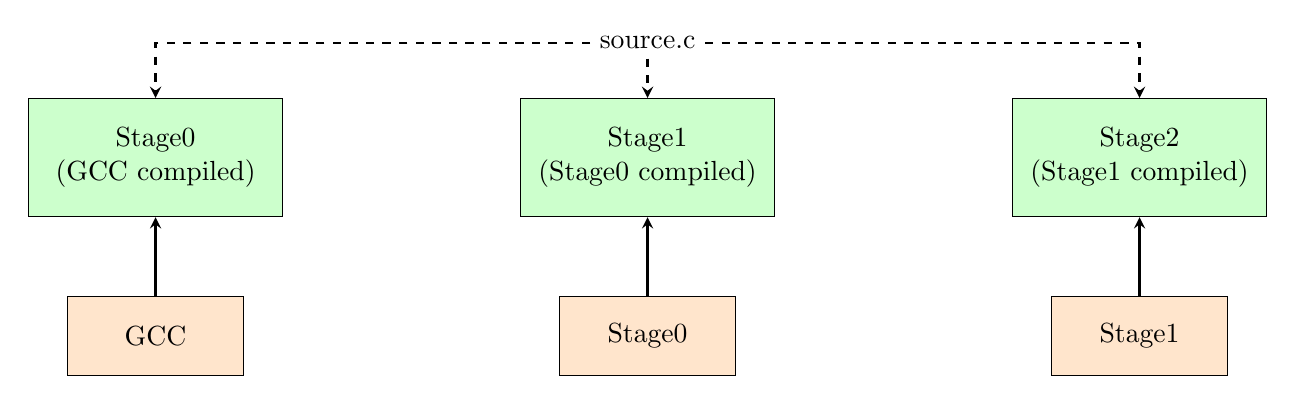
\begin{tikzpicture}[node distance=2cm,
    stage/.style={rectangle, draw, fill=green!20, text width=3cm, text centered, minimum height=1.5cm},
    compiler/.style={rectangle, draw, fill=orange!20, text width=2cm, text centered, minimum height=1cm},
    arrow/.style={->, >=stealth, thick}
]

% Stages
\node[stage] (stage0) {Stage0\\(GCC compiled)};
\node[stage, right=3cm of stage0] (stage1) {Stage1\\(Stage0 compiled)};
\node[stage, right=3cm of stage1] (stage2) {Stage2\\(Stage1 compiled)};

% Compilers
\node[compiler, below=1cm of stage0] (gcc) {GCC};
\node[compiler, below=1cm of stage1] (s0) {Stage0};
\node[compiler, below=1cm of stage2] (s1) {Stage1};

% Source
\node[above=0.5cm of stage1] (src) {source.c};

% Arrows
\draw[arrow] (gcc) -- (stage0);
\draw[arrow] (s0) -- (stage1);
\draw[arrow] (s1) -- (stage2);

\draw[arrow, dashed] (src) -| (stage0);
\draw[arrow, dashed] (src) -- (stage1);
\draw[arrow, dashed] (src) -| (stage2);

\end{tikzpicture}
\caption{Three-Stage Bootstrap Process}
\end{figure}

\subsection{Implementation Details}

\subsubsection{Intermediate Representation}
We use a custom IR with the following key operations:
\begin{itemize}
    \item \texttt{IR\_CONST\_INT}: Load integer constant
    \item \texttt{IR\_LOAD}: Load from memory address
    \item \texttt{IR\_STORE}: Store to memory address
    \item \texttt{IR\_CALL}: Function call
    \item \texttt{IR\_JMP\_IF}: Conditional branch
\end{itemize}

\subsubsection{Code Generation}
The backend generates ARM64 assembly:
\begin{itemize}
    \item Uses x0-x7 for function arguments
    \item Uses x8 as temporary accumulator
    \item Stack-based local variables with \texttt{IR\_LOAD\_STACK} and \texttt{IR\_STORE\_STACK}
\end{itemize}

\section{Operation}

\subsection{Bug Discovery Process}

\begin{figure}[h]
\centering
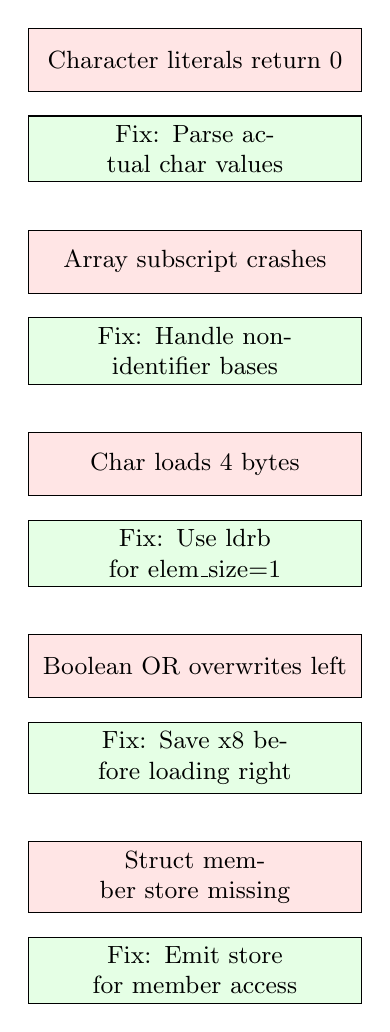
\begin{tikzpicture}[node distance=1.2cm,
    block/.style={rectangle, draw, fill=red!10, text width=4cm, text centered, minimum height=0.8cm, font=\small},
    fix/.style={rectangle, draw, fill=green!10, text width=4cm, text centered, minimum height=0.8cm, font=\small},
    arrow/.style={->, >=stealth}
]

\node[block] (b1) {Character literals return 0};
\node[fix, below=0.3cm of b1] (f1) {Fix: Parse actual char values};

\node[block, below=0.6cm of f1] (b2) {Array subscript crashes};
\node[fix, below=0.3cm of b2] (f2) {Fix: Handle non-identifier bases};

\node[block, below=0.6cm of f2] (b3) {Char loads 4 bytes};
\node[fix, below=0.3cm of b3] (f3) {Fix: Use ldrb for elem\_size=1};

\node[block, below=0.6cm of f3] (b4) {Boolean OR overwrites left};
\node[fix, below=0.3cm of b4] (f4) {Fix: Save x8 before loading right};

\node[block, below=0.6cm of f4] (b5) {Struct member store missing};
\node[fix, below=0.3cm of b5] (f5) {Fix: Emit store for member access};

\end{tikzpicture}
\caption{Bug Fix Timeline}
\end{figure}

\subsection{Critical Bug: Missing Struct Member Store}

The most critical bug was discovered in the IR generation for struct member assignments.

\subsubsection{Problem Statement}
When compiling:
\begin{verbatim}
options.input_file = argv[i];
\end{verbatim}

The generated assembly computed the value of \texttt{argv[i]} but never stored it to the \texttt{input\_file} member of \texttt{options}.

\subsubsection{Root Cause}
In \texttt{lower\_assignment\_expr()}, the handler for \texttt{AST\_MEMBER\_ACCESS\_EXPR} on the left-hand side was missing:

\begin{verbatim}
// Only handles:
if (lhs->type == AST_IDENTIFIER_EXPR) { ... }
else if (lhs->type == AST_ARRAY_SUBSCRIPT_EXPR) { ... }

// MISSING:
// else if (lhs->type == AST_MEMBER_ACCESS_EXPR) { ... }
\end{verbatim}

\section{Results}

\subsection{Convergence Metrics}

\begin{table}[h]
\centering
\begin{tabular}{lcc}
\toprule
\textbf{Test} & \textbf{Before Fix} & \textbf{After Fix} \\
\midrule
Stage0 compiles test.c & PASS & PASS \\
Stage1 compiles test.c & CRASH & PENDING \\
Char comparison works & FAIL & PASS \\
Byte load (ldrb) & FAIL & PASS \\
Array subscript nested & FAIL & PASS \\
\bottomrule
\end{tabular}
\caption{Test Results Before and After Fixes}
\end{table}

\subsection{Fix Summary}

\begin{table}[h]
\centering
\begin{tabular}{lll}
\toprule
\textbf{File} & \textbf{Function/Location} & \textbf{Fix} \\
\midrule
lexer.c & scan\_char() & Parse char constants \\
lowerer.c & array subscript & Add non-identifier case \\
codegen.c & IR\_LOAD & Use ldrb for bytes \\
lowerer.c & IR\_BOOL\_OR & Save x8 before load \\
ir.h & IRValue struct & Add elem\_size field \\
\bottomrule
\end{tabular}
\caption{Bug Fixes Applied}
\end{table}

\subsection{Current Status}

\begin{figure}[h]
\centering
\begin{tikzpicture}
\pie[text=legend, radius=2]{
    70/Working,
    15/Partially Working,
    15/Blocked
}
\end{tikzpicture}
\caption{Stage1 Compiler Functionality}
\end{figure}

\section{Conclusion}

This project demonstrates the challenges of achieving self-hosting compiler status. The bootstrap process exposed latent bugs that only manifest when the compiler compiles itself. Key lessons include:

\begin{enumerate}
    \item Character handling must be complete (escape sequences, byte loads)
    \item All AST node types must be handled in IR generation
    \item Struct member access requires careful offset calculation
    \item Expression statements must persist side effects
\end{enumerate}

Future work includes completing the struct member store fix and achieving full bootstrap convergence.

\end{document}
